\documentclass[11pt,a4paper]{article}
\usepackage[utf8]{inputenc}
\usepackage{amsmath,amsfonts,amssymb}
\usepackage{graphicx}
\usepackage{geometry}
\geometry{margin=1in}
\usepackage{booktabs}
\usepackage{hyperref}
\usepackage{float}
\usepackage{xcolor}

\definecolor{darkbg}{HTML}{0d121f}
\definecolor{lighttext}{HTML}{e2e8f0}
\definecolor{primary}{HTML}{8b5cf6}
\definecolor{secondary}{HTML}{0dd5c5}
\definecolor{accent}{HTML}{10b981}

\pagecolor{darkbg}
\color{lighttext}

\hypersetup{
    colorlinks=true,
    linkcolor=secondary,
    urlcolor=secondary,
    citecolor=accent
}

\title{\textbf{EE3621: Digital Signal Processing} \\ \Large Lecture 27: Matched-Z IIR Design Example and the Adaptive Filter Framework (Wiener Solution \& LMS) \\ \large (III B.Tech EEE)}
\author{Comprehensive Lecture Notes \& Faculty Textbook Reference}
\date{}

\begin{document}

\maketitle

\noindent\rule{\textwidth}{0.5pt}

\section*{Lecture Plan \& Objectives (40 Minutes Breakdown)}
\begin{itemize}
    \item \textbf{00:00 -- 05:00 (5 mins):} Recap: analog-to-digital IIR conversion and the pole-mapping $z = e^{sT}$; why zeros ``at infinity'' need special care.
    \item \textbf{05:00 -- 20:00 (15 mins):} Worked Design (Example 27.1): digital filter from $H_a(s) = \frac{2}{(s+1)(s+2)}$ with $T = 0.1$\,s --- pole/zero bookkeeping, pole mapping, zeros placed at $z=-1$, DC-gain matching.
    \item \textbf{20:00 -- 27:00 (7 mins):} The Adaptive Filter Framework: input $x[n]$, desired $d[n]$, output $y[n]$, error $e[n]$, update algorithm (block diagram).
    \item \textbf{27:00 -- 35:00 (8 mins):} Mathematics: input/weight vectors, MSE cost $J(\mathbf{w})$, normal equations (Wiener solution), and the Widrow--Hoff LMS update.
    \item \textbf{35:00 -- 40:00 (5 mins):} Worked LMS iteration (Example 27.2), pitfalls, and a teaser for Lecture 28 (why this is already machine learning).
\end{itemize}

\noindent\rule{\textwidth}{0.5pt}

\section{1. LEARNING OBJECTIVES}
By the end of this lecture, students will be able to:
\begin{enumerate}
    \item \textbf{Count} the poles, finite zeros and zeros at infinity of an analog prototype ($N$, $M$, $N-M$).
    \item \textbf{Map} analog poles to the $z$-plane using $p_k \mapsto e^{p_k T}$ and \textbf{place} the $N-M$ missing zeros at $z=-1$.
    \item \textbf{Match} the DC gain of the digital filter to the analog prototype by computing a scale factor $K_d$.
    \item \textbf{Draw} the adaptive filter block diagram and identify $x[n]$, $d[n]$, $y[n]$, $e[n]$ and the update block.
    \item \textbf{Write} the MSE cost $J(\mathbf{w}) = E[d^2] - 2\mathbf{w}^T\mathbf{p} + \mathbf{w}^T\mathbf{R}\mathbf{w}$ and its minimizer $\mathbf{w}^\ast = \mathbf{R}^{-1}\mathbf{p}$.
    \item \textbf{Derive} the LMS recursion $\mathbf{w}^{(i+1)} = \mathbf{w}^{(i)} + \mu\, e[n]\,\mathbf{x}[n]$ (tap-by-tap: $w_k^{(i+1)} = w_k^{(i)} + \mu\, e[n]\, x[n-k]$) from an instantaneous gradient estimate.
    \item \textbf{Disambiguate} clearly between discrete-time index $n$, filter tap index $k$, and adaptation iteration step $i$.
\end{enumerate}

\noindent\rule{\textwidth}{0.5pt}

\section{2. IIR DESIGN BY POLE MAPPING WITH ZEROS AT $z=-1$}

\subsection{2.1 Idea}
A strictly proper analog filter $H_a(s)$ with $N$ poles and $M < N$ finite zeros has $N-M$ zeros at $s=\infty$. Under the mapping $z = e^{sT}$:
\begin{itemize}
    \item each pole $p_k$ maps to $z_k = e^{p_k T}$ (stable $\Rightarrow$ $|z_k|<1$);
    \item each finite zero $q_k$ maps to $e^{q_k T}$;
    \item the $N-M$ zeros at $s \to \infty$ correspond to the highest analog frequency, $\Omega = \pi/T$, i.e.\ to $\omega = \pi$, i.e.\ to $z=-1$. We therefore \textbf{insert $(N-M)$ zeros at $z=-1$}, i.e.\ factors $(1+z^{-1})^{N-M}$.
\end{itemize}
Because pole/zero mapping does not preserve gain, the result is scaled by a constant $K_d$ so that the DC gains agree: $H(1) = H_a(0)$.

\subsection{2.2 Procedure}
\begin{enumerate}
    \item Identify poles ($N$), finite zeros ($M$), zeros at infinity ($N-M$).
    \item Map all poles and finite zeros with $e^{(\cdot)T}$.
    \item Add $N-M$ zeros at $z=-1$ to form the unscaled filter $H''(z)$.
    \item Compute $K_d = H_a(0)/H''(1)$ and set $H(z) = K_d\,H''(z)$.
\end{enumerate}

\section{3. WORKED EXAMPLE 27.1 -- SECOND-ORDER LOWPASS}

\noindent\textbf{Problem:} Design a digital filter from the 2nd-order analog lowpass
\begin{equation}
H_a(s) = \frac{2}{(s+1)(s+2)}, \qquad T = 0.1\ \text{s}.
\end{equation}

\noindent\textbf{Step 1: Poles, zeros and degrees.}
\begin{itemize}
    \item Poles: $p_1 = -1$, $p_2 = -2 \implies N = 2$.
    \item Finite zeros: none ($M=0$).
    \item Zeros at infinity: $N - M = 2 - 0 = 2$.
\end{itemize}

\noindent\textbf{Step 2: Map poles; add zeros at $z=-1$.}
\begin{align}
e^{p_1 T} &= e^{-1\times 0.1} = e^{-0.1} \approx 0.9048 \\
e^{p_2 T} &= e^{-2\times 0.1} = e^{-0.2} \approx 0.8187
\end{align}
Two zeros are added at $z=-1$, giving $(1+z^{-1})^2$. The unscaled digital transfer function is
\begin{equation}
H''(z) = \frac{(1+z^{-1})^2}{(1 - 0.9048\,z^{-1})(1 - 0.8187\,z^{-1})}.
\end{equation}

\noindent\textbf{Step 3: Match the DC gain.} For the analog filter at $s=0$:
\begin{equation}
H_a(0) = \frac{2}{(0+1)(0+2)} = 1.
\end{equation}
For the unscaled digital filter at $z=1$ ($z^{-1}=1$):
\begin{equation}
H''(1) = \frac{(1+1)^2}{(1-0.9048)(1-0.8187)} = \frac{4}{(0.0952)(0.1813)} \approx \frac{4}{0.01726} \approx 231.75.
\end{equation}
To force $H(1) = 1$:
\begin{equation}
K_d = \frac{H_a(0)}{H''(1)} = \frac{1}{231.75} \approx 0.004315.
\end{equation}

\noindent\textbf{Result:}
\begin{equation}
\boxed{H(z) = \frac{0.004315\,(1+z^{-1})^2}{(1 - 0.9048\,z^{-1})(1 - 0.8187\,z^{-1})}}
\end{equation}

\noindent\textbf{Difference equation.} Expanding the denominator, $(1-0.9048z^{-1})(1-0.8187z^{-1}) = 1 - 1.7235\,z^{-1} + 0.7408\,z^{-2}$, and the numerator $0.004315(1 + 2z^{-1} + z^{-2})$, so
\begin{equation}
y[n] = 1.7235\,y[n-1] - 0.7408\,y[n-2] + 0.004315\big(x[n] + 2x[n-1] + x[n-2]\big).
\end{equation}

\begin{figure}[H]
\centering
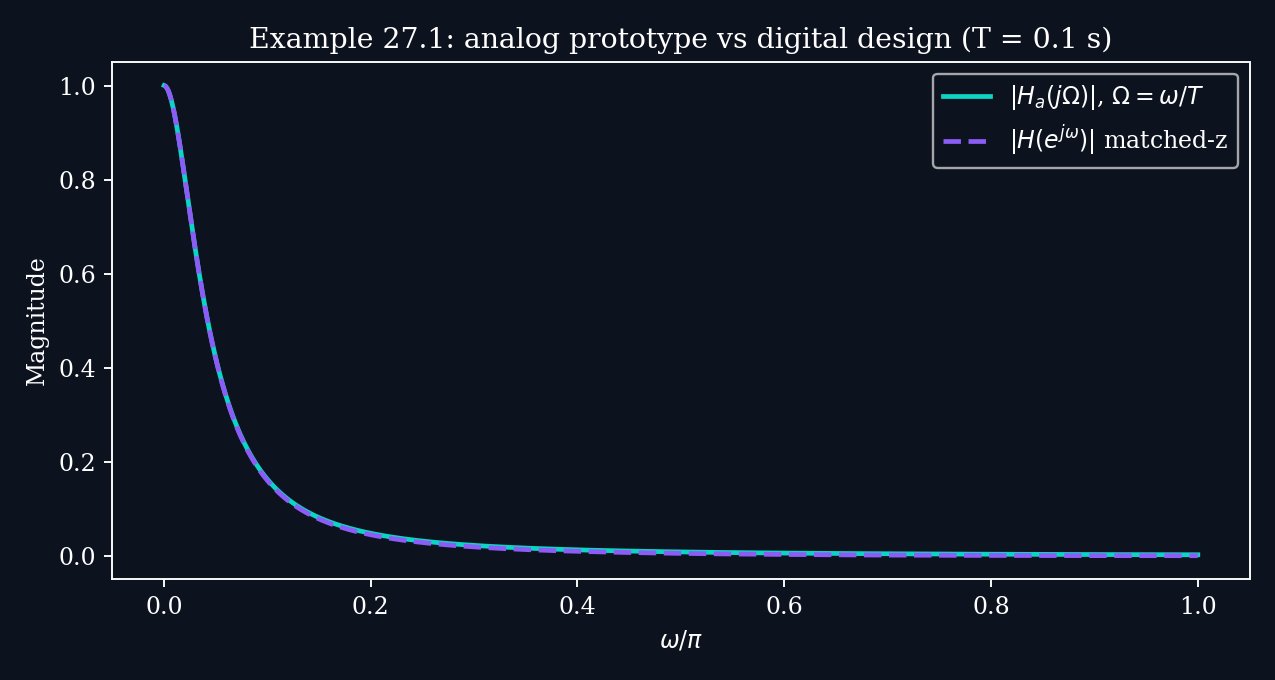
\includegraphics[width=0.8\textwidth]{images/l27_matchedz_response.png}
\caption{Magnitude of the analog prototype versus the digital filter of Example 27.1. The double zero at $z=-1$ drives the digital response to zero at $\omega=\pi$ whereas the analog response is only small ($\approx 0.002$ at $\Omega=\pi/T$).}
\end{figure}

\noindent\textbf{Check:} $|H(e^{j0})| \approx 1.000$, and $|H(e^{j\pi})| = 0$ because of the zeros at $z=-1$.

\subsection{3.1 Design remarks}
\begin{itemize}
    \item The pole mapping is exact for the poles but the \emph{frequency response} is only approximate: this is not a bilinear transform, and aliasing is not eliminated. It works well when $|H_a(j\Omega)|$ is already small near $\Omega = \pi/T$ (here $T=0.1$ gives $\pi/T \approx 31.4$ rad/s, far beyond the poles at 1 and 2 rad/s).
    \item Choose $T$ small compared with the inverse of the fastest pole; if $T$ were $1$\,s the poles would map to $0.37$ and $0.14$ and the match would deteriorate.
    \item Always \emph{match the gain at a chosen reference frequency}; DC is natural for lowpass filters.
\end{itemize}

\noindent\rule{\textwidth}{0.5pt}

\section{4. THE ADAPTIVE FILTER FRAMEWORK}

Everything so far (Lectures 15--27) designed \textbf{fixed} coefficients from a known specification. An \textbf{adaptive filter} instead \emph{learns} its coefficients from data, by comparing its output with a desired signal.

\begin{figure}[H]
\centering
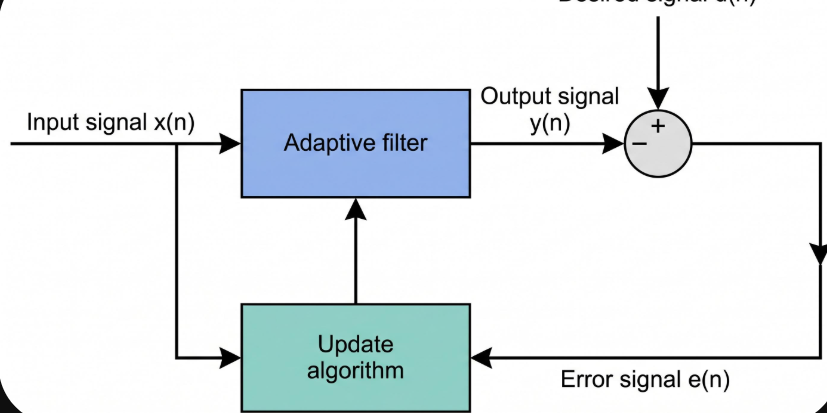
\includegraphics[width=0.75\textwidth]{images/l27_adaptive_block.png}
\caption{Adaptive filter: the filter output $y[n]$ is subtracted from the desired signal $d[n]$; the error $e[n]$ and the input $x[n]$ drive the update algorithm that adjusts the filter coefficients.}
\end{figure}

\begin{center}
\resizebox{\textwidth}{!}{
\begin{tabular}{lll}
\toprule
\textbf{Variable / Signal} & \textbf{Role in Framework} & \textbf{Domain / Index Range} \\
\midrule
$n$ & Discrete-time sample index & $n \in \{0, 1, 2, \dots\}$ \\
$k$ & Filter tap index (delay stage) & $k \in \{0, 1, \dots, M-1\}$ \\
$i$ & Adaptation iteration step & $i \in \{0, 1, 2, \dots\}$ \\
$x[n]$ & Input reference signal & Sample arriving at time $n$ \\
$d[n]$ & Desired (target) response & Reference signal at time $n$ \\
$y^{(i)}[n]$ & Adaptive filter output & Transversal sum at time $n$ for iteration $i$ \\
$e^{(i)}[n] = d[n]-y^{(i)}[n]$ & Instantaneous estimation error & Drives coefficient update at iteration $i$ \\
$w_k^{(i)}$ & Weight of tap $k$ at iteration $i$ & Adaptive filter coefficient \\
\bottomrule
\end{tabular}
}
\end{center}

\subsection{4.1 Vector Notation \& Index Disambiguation}
In classical DSP textbooks, the symbol $n$ is frequently overloaded to represent both physical discrete time ($x[n]$) and the optimization iteration counter ($w_k[n]$). To eliminate confusion between the \textbf{tap position ($k$)}, the \textbf{time sample ($n$)}, and the \textbf{algorithm iteration ($i$)}:
\begin{itemize}
    \item $k \in \{0, 1, \dots, M-1\}$ is the \textbf{spatial / tap index} along the FIR tapped delay line.
    \item $n$ is the \textbf{discrete-time sample index} of the continuous signal streams $x[n]$ and $d[n]$.
    \item $i$ is the \textbf{adaptation iteration index} ($i = 0, 1, 2, \dots$). In sample-by-sample LMS, iteration $i$ processes sample $n = i$.
\end{itemize}

\noindent At discrete time $n$, the $M$-tap input delay line stores the current and past input samples:
\begin{equation}
\mathbf{x}[n] = \big[x[n],\; x[n-1],\; \dots,\; x[n-M+1]\big]^T \quad \text{($M \times 1$ input vector)}
\end{equation}
The adaptive filter coefficients at iteration $i$ form the weight vector:
\begin{equation}
\mathbf{w}^{(i)} = \big[w_0^{(i)},\; w_1^{(i)},\; \dots,\; w_{M-1}^{(i)}\big]^T \quad \text{($M \times 1$ weight vector)}
\end{equation}
\textbf{Filter output at sample $n$ using weights of iteration $i$:}
\begin{equation}
y^{(i)}[n] = \big(\mathbf{w}^{(i)}\big)^T \mathbf{x}[n] = \sum_{k=0}^{M-1} w_k^{(i)}\,x[n-k].
\end{equation}
Notice the clean separation: the sum is taken over the tap index $k$, multiplying the $k$-th tap weight $w_k^{(i)}$ by the delayed input sample $x[n-k]$.

\subsubsection*{Representation Note: Why $y^{(i)}[n], e^{(i)}[n]$ Depend on $i$, and When $x^{(i)}[n], d^{(i)}[n]$ Are Used}

\noindent\textbf{1. Why $y^{(i)}[n]$ and $e^{(i)}[n]$ carry the iteration index $(i)$:} \\
The filter output $y^{(i)}[n] = \sum_{k=0}^{M-1} w_k^{(i)} x[n-k]$ and estimation error $e^{(i)}[n] = d[n] - y^{(i)}[n]$ \textbf{depend directly on the adaptive weights $\mathbf{w}^{(i)}$}. Because the weights adapt from iteration to iteration ($i \to i+1$), the output and error change dynamically at every learning step even when evaluated on the same sample $n$. Writing $y^{(i)}[n]$ and $e^{(i)}[n]$ explicitly tracks this progressive learning process.

\vspace{2mm}
\noindent\textbf{2. When are $x^{(i)}[n]$ and $d^{(i)}[n]$ used? (Validity and Physical Context)}
\begin{itemize}
    \item \textbf{Online Sample-by-Sample LMS (Single Continuous Stream):}
    Here, $x[n]$ and $d[n]$ are generated by external physical processes (e.g., continuous sensor/microphone signals). Since discrete time increments with each sample step ($n = i$), the input at sample $n$ is fixed and independent of the filter's learning iteration. Therefore, writing $x^{(i)}[n]$ or $d^{(i)}[n]$ in standard single-stream LMS is \textbf{redundant}, and standard notation uses simply $x[n]$ and $d[n]$.
    
    \item \textbf{When $x^{(i)}[n]$ and $d^{(i)}[n]$ ARE Valid and Standard in DSP:}
    When the input or desired data sequences themselves change with each iteration $i$, using $x^{(i)}[n]$ and $d^{(i)}[n]$ is mathematically exact. Two major DSP formulations use this:
    \begin{enumerate}
        \item \textbf{Representation 1: Block / Frame-Based Processing (Block LMS):}
        A continuous signal is split into consecutive blocks (frames) of length $L$. Here, $i$ is the \textbf{block/frame iteration index} ($i = 0, 1, 2, \dots$), and $n$ is the \textbf{sample index within that block} ($n = 0, 1, \dots, L-1$). The input and desired data change with each block iteration:
        \begin{equation}
        x^{(i)}[n] = x[i \cdot L + n], \qquad d^{(i)}[n] = d[i \cdot L + n].
        \end{equation}
        The filter computes $y^{(i)}[n] = \sum_{k=0}^{M-1} w_k^{(i)} x^{(i)}[n-k]$ and error $e^{(i)}[n] = d^{(i)}[n] - y^{(i)}[n]$ over the block, and the weights $\mathbf{w}^{(i+1)}$ update once per frame.
        
        \item \textbf{Representation 2: Multi-Trial / Repetitive Sweep Processing (Ensemble LMS):}
        In biomedical signal processing (e.g., EEG/ECG evoked responses), radar/sonar chirps, and machine learning epochs, an experiment is repeated across multiple trials. Here, $i$ is the \textbf{trial / sweep / run number} ($i = 1, 2, \dots$), and $n$ is the \textbf{elapsed time relative to the stimulus trigger} ($n = 0, 1, \dots, T-1$). Because background noise $v^{(i)}[n]$ and physical channel conditions vary from trial to trial:
        \begin{equation}
        x^{(i)}[n] = s[n] + v^{(i)}[n], \qquad d^{(i)}[n] = \text{Target response in trial } i.
        \end{equation}
        The input and desired waveforms genuinely differ across iterations $i$ due to trial-specific noise realizations.
    \end{enumerate}
\end{itemize}

\subsection{4.2 Error and cost function}
\begin{equation}
e^{(i)}[n] = d[n] - y^{(i)}[n]
\end{equation}
\textbf{Mean-square-error cost} (with fixed $\mathbf{w}$):
\begin{equation}
J(\mathbf{w}) = E[e^2[n]] = E[d^2[n]] - 2\mathbf{w}^T\mathbf{p} + \mathbf{w}^T\mathbf{R}\,\mathbf{w}
\end{equation}
where $\mathbf{R} = E[\mathbf{x}[n]\mathbf{x}^T[n]]$ is the input autocorrelation matrix and $\mathbf{p} = E[d[n]\,\mathbf{x}[n]]$ is the cross-correlation vector.

\textbf{Wiener solution.} $J$ is a quadratic bowl in $\mathbf{w}$. Its gradient is
\begin{equation}
\nabla J = -2\mathbf{p} + 2\mathbf{R}\mathbf{w}.
\end{equation}
Setting $\nabla J = \mathbf{0}$ gives the normal (Wiener--Hopf) equations
\begin{equation}
\mathbf{R}\,\mathbf{w}^\ast = \mathbf{p} \implies \mathbf{w}^\ast = \mathbf{R}^{-1}\mathbf{p}.
\end{equation}
Computing this directly requires knowing $\mathbf{R}$ and $\mathbf{p}$ and inverting $\mathbf{R}$ --- unrealistic in real time, hence LMS.

\subsection{4.3 The Widrow--Hoff LMS Algorithm}
Replace the true gradient by an instantaneous estimate from the current sample $n$:
\begin{equation}
\hat{\nabla} J^{(i)}[n] = \frac{\partial (e^{(i)}[n])^2}{\partial \mathbf{w}} = 2e^{(i)}[n]\frac{\partial e^{(i)}[n]}{\partial \mathbf{w}} = -2e^{(i)}[n]\,\mathbf{x}[n].
\end{equation}
Stepping in the negative gradient direction (absorbing the factor $2$ into step size $\mu$), the weight vector updates from iteration $i$ to $i+1$:
\begin{equation}
\boxed{\mathbf{w}^{(i+1)} = \mathbf{w}^{(i)} + \mu\, e^{(i)}[n]\,\mathbf{x}[n]}
\end{equation}
In scalar form, updating each individual tap weight $k \in \{0, 1, \dots, M-1\}$:
\begin{equation}
\boxed{w_k^{(i+1)} = w_k^{(i)} + \mu\, e^{(i)}[n]\, x[n-k]}
\end{equation}
\begin{itemize}
    \item \textbf{Textbook notation equivalence:} In classical texts where iteration is denoted as $n$ instead of $i$, this equation is written as $\mathbf{w}[n+1] = \mathbf{w}[n] + \mu e[n]\mathbf{x}[n]$ and $w_k[n+1] = w_k[n] + \mu e[n]x[n-k]$. Introducing $i$ clarifies that $i$ is the iteration count, $n$ is discrete time, and $k$ is the tap index.
    \item \textbf{Convention note:} Lecture 26 wrote $\mathbf{w}^{(i+1)} = \mathbf{w}^{(i)} + 2\mu\, e[n]\mathbf{x}[n]$. The two forms are identical with $\mu_{27} = 2\mu_{26}$. Always check which convention an exam question uses.
    \item With this convention, mean convergence requires $0 < \mu < 2/\lambda_{\max}(\mathbf{R})$, and the practical sufficient condition is $0 < \mu < 2/(M P_x)$, since $\lambda_{\max} \le \mathrm{Tr}(\mathbf{R}) = M P_x$.
\end{itemize}

\begin{figure}[H]
\centering
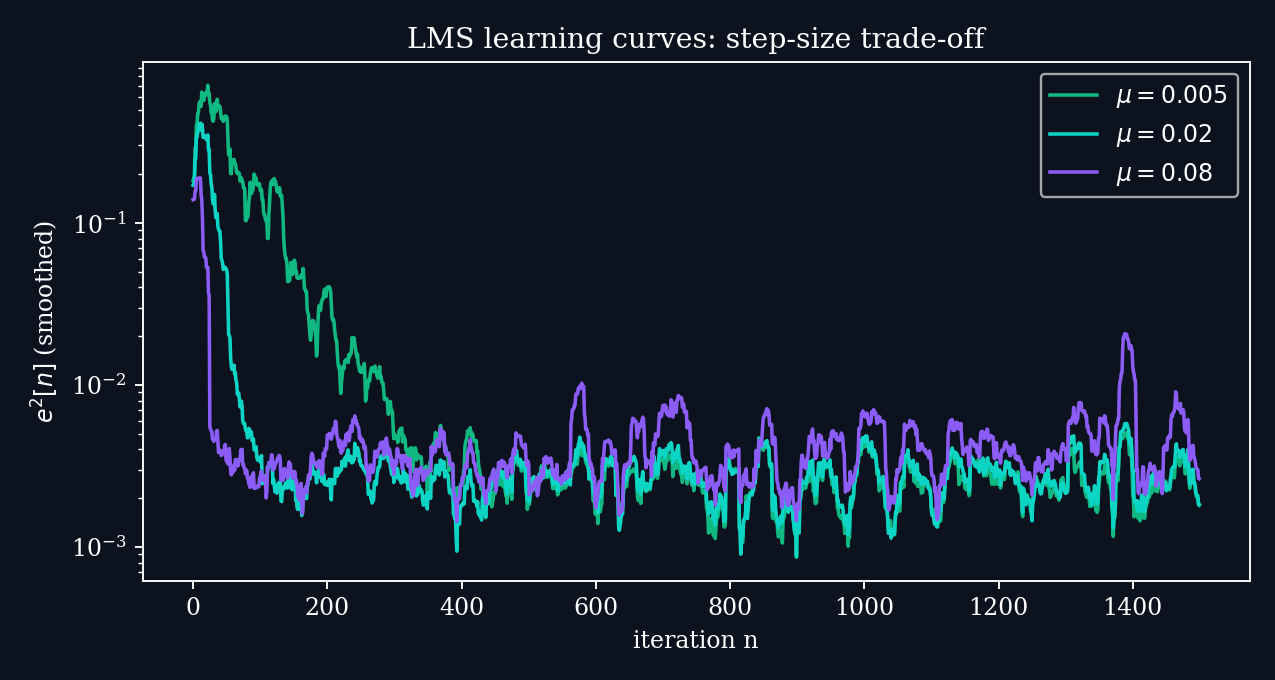
\includegraphics[width=0.8\textwidth]{images/l27_lms_curves.png}
\caption{LMS system identification of a 4-tap FIR system with three step sizes (convention $\mathbf{w} \leftarrow \mathbf{w} + 2\mu e\mathbf{x}$): large $\mu$ converges fast but leaves more steady-state error; small $\mu$ is slow but accurate.}
\end{figure}

\subsection{4.4 Algorithmic Pseudocode (LMS Adaptive FIR Filter)}
The following pseudocode outlines the complete sample-by-sample LMS implementation, making the separation between the iteration loop ($i$), tap index ($k$), and sample time ($n$) explicit:

\begin{verbatim}
========================================================================
ALGORITHM: Sample-by-Sample LMS Adaptive FIR Filter
========================================================================
Inputs:
  x[n]      : Input signal stream of length N_samples (n = 0, ..., N - 1)
  d[n]      : Desired target stream of length N_samples (n = 0, ..., N - 1)
  M         : Number of filter taps (filter order = M - 1)
  mu        : Step-size parameter (learning rate)
Outputs:
  y[n]      : Adaptive filter output stream
  e[n]      : Estimation error stream
  w_k^(end) : Final converged tap weights

1. INITIALIZATION:
   For k = 0 to M - 1:
       w[k]      = 0.0      // Initial tap weight w_k^(0) = 0 for tap k
       buffer[k] = 0.0      // Delay line buffer: holds [x[n], ..., x[n-M+1]]

2. ADAPTATION LOOP (Iteration index i = 0, 1, 2, ..., N_samples - 1):
   For i = 0 to N_samples - 1:
       n = i                // Current time sample matches iteration index

       // Step A: Shift delay line buffer & insert incoming sample x[n]
       For k = M - 1 down to 1:
           buffer[k] = buffer[k - 1]
       buffer[0] = x[n]     // buffer[k] now contains delayed sample x[n-k]

       // Step B: Transversal Filter Output (Summation over tap index k)
       y[n] = 0.0
       For k = 0 to M - 1:
           y[n] = y[n] + ( w[k] * buffer[k] )

       // Step C: Instantaneous Estimation Error
       e[n] = d[n] - y[n]   // Computes error e^(i)[n]

       // Step D: LMS Tap Weight Update (Transition: iteration i -> i + 1)
       For k = 0 to M - 1:
           // w_k^(i+1) = w_k^(i) + mu * e^(i)[n] * x[n-k]
           w[k] = w[k] + ( mu * e[n] * buffer[k] )

   End For
========================================================================
\end{verbatim}

\noindent\rule{\textwidth}{0.5pt}

\section{5. WORKED EXAMPLE 27.2 -- TWO LMS ITERATIONS}

\textbf{Problem:} Given initial weight vector at iteration $i=0$: $\mathbf{w}^{(0)} = [0,\;0]^T$ ($M=2$ taps, $k \in \{0, 1\}$), step size $\mu = 0.1$, and update rule $w_k^{(i+1)} = w_k^{(i)} + \mu e^{(i)}[n] x[n-k]$, process the two input/desired pairs:
\[
\mathbf{x}[0] = [x[0],\; x[-1]]^T = [1.0,\; 0.5]^T,\quad d[0] = 2.0;
\]
\[
\mathbf{x}[1] = [x[1],\; x[0]]^T  = [0.5,\; 1.0]^T,\quad d[1] = 1.5.
\]

\noindent\textbf{Iteration $i=0$ (Processing sample $n=0$):}
\begin{align}
y^{(0)}[0] &= w_0^{(0)} x[0] + w_1^{(0)} x[-1] = (0)(1.0) + (0)(0.5) = 0 \\
e^{(0)}[0] &= d[0] - y^{(0)}[0] = 2.0 - 0 = 2.0 \\
\text{Tap } k=0: \quad w_0^{(1)} &= w_0^{(0)} + \mu\, e^{(0)}[0]\, x[0] = 0 + (0.1)(2.0)(1.0) = \mathbf{0.20} \\
\text{Tap } k=1: \quad w_1^{(1)} &= w_1^{(0)} + \mu\, e^{(0)}[0]\, x[-1] = 0 + (0.1)(2.0)(0.5) = \mathbf{0.10}
\end{align}
The updated weight vector for iteration $i=1$ is $\mathbf{w}^{(1)} = [0.20,\; 0.10]^T$.

\vspace{2mm}
\noindent\textbf{Iteration $i=1$ (Processing sample $n=1$):}
\begin{align}
y^{(1)}[1] &= w_0^{(1)} x[1] + w_1^{(1)} x[0] = (0.20)(0.5) + (0.10)(1.0) = 0.20 \\
e^{(1)}[1] &= d[1] - y^{(1)}[1] = 1.5 - 0.20 = \mathbf{1.30} \\
\text{Tap } k=0: \quad w_0^{(2)} &= w_0^{(1)} + \mu\, e^{(1)}[1]\, x[1] = 0.20 + (0.1)(1.30)(0.5) = \mathbf{0.265} \\
\text{Tap } k=1: \quad w_1^{(2)} &= w_1^{(1)} + \mu\, e^{(1)}[1]\, x[0] = 0.10 + (0.1)(1.30)(1.0) = \mathbf{0.230}
\end{align}
The updated weight vector for iteration $i=2$ is $\mathbf{w}^{(2)} = [0.265,\; 0.230]^T$. The weights adjust along the gradient to progressively minimize output error.

\noindent\rule{\textwidth}{0.5pt}

\section{6. FACULTY INSIGHTS, PITFALLS \& EXAM TRAPS}
\begin{itemize}
    \item \textbf{Index Confusion ($n$ vs.\ $k$ vs.\ $i$):} The most common exam trap is mixing up the filter tap index $k$ ($0 \le k \le M-1$) with the discrete time $n$ or iteration count $i$. In $w_k^{(i)}$, $k$ chooses the physical tap multiplier, while $i$ indexes the training iteration. When updating tap $k$, always multiply the error $e[n]$ by the sample present at tap $k$, which is $x[n-k]$ (not $x[n]$ or $x[k]$!).
    \item \textbf{Forgetting the zeros at $z=-1$:} the filter then has fewer zeros than poles and the high-frequency attenuation is wrong. Always compute $N-M$.
    \item \textbf{Forgetting $K_d$:} the unscaled $H''(1)$ is $\approx 231.75$, a gain of $47$\,dB!
    \item \textbf{Wrong direction of the update:} the update is $+\mu e\mathbf{x}$ because the gradient estimate is $-2e\mathbf{x}$.
    \item \textbf{Mixing $2\mu$ and $\mu$ conventions} (see \S 4.3).
    \item \textbf{Using $x[n]$ vs.\ $d[n]$ in the update:} LMS multiplies the \emph{error} by the \emph{input vector}; $d[n]$ only enters through $e[n]$.
\end{itemize}

\vspace{2mm}
\noindent\textbf{Looking ahead (Lecture 28):} The LMS equation is, symbol for symbol, the delta rule used to train a single artificial neuron. The next lecture maps DSP onto machine learning systematically.

\noindent\rule{\textwidth}{0.5pt}

\section{7. QUICK REVISION CHEAT-SHEET}
\begin{table}[H]
\centering
\resizebox{\textwidth}{!}{
\begin{tabular}{lll}
\toprule
\textbf{Topic} & \textbf{Formula} & \textbf{Note} \\
\midrule
Pole mapping & $p_k \mapsto e^{p_k T}$ & stable $\to$ inside unit circle \\
Zeros at $\infty$ & $(1+z^{-1})^{N-M}$ & $s=\infty \leftrightarrow z=-1$ \\
DC gain match & $K_d = H_a(0)/H''(1)$ & $K_d = 0.004315$ in Ex.\ 27.1 \\
Index distinction & $k = \text{tap},\; n = \text{time},\; i = \text{iteration}$ & Avoids variable overloading \\
Filter Output & $y^{(i)}[n] = (\mathbf{w}^{(i)})^T\mathbf{x}[n] = \sum_{k=0}^{M-1} w_k^{(i)} x[n-k]$ & Output depends on weights at step $i$ \\
Estimation Error & $e^{(i)}[n] = d[n] - y^{(i)}[n]$ & Drives weight updates at step $i$ \\
Signal context & $x^{(i)}[n], d^{(i)}[n]$ used in Block/Trial LMS & Redundant in sample-by-sample ($n=i$) \\
Cost function & $J = E[d^2] - 2\mathbf{w}^T\mathbf{p} + \mathbf{w}^T\mathbf{R}\mathbf{w}$ & Quadratic error bowl \\
Wiener solution & $\mathbf{w}^\ast = \mathbf{R}^{-1}\mathbf{p}$ & Optimal MMSE solution \\
LMS Vector Update & $\mathbf{w}^{(i+1)} = \mathbf{w}^{(i)} + \mu e^{(i)}[n]\mathbf{x}[n]$ & Iteration step $i \to i+1$ \\
LMS Tap Update & $w_k^{(i+1)} = w_k^{(i)} + \mu e^{(i)}[n] x[n-k]$ & Tap $k$ updated by delayed sample $x[n-k]$ \\
\bottomrule
\end{tabular}
}
\end{table}

\end{document}
